\documentclass[convert={ghostscript,gsdevice=tiffg4,
outext=.tiff,density=1200}]{standalone}
    \usepackage{tikz}
    \usepackage{pgfplots}
    \usetikzlibrary{patterns}
\mathversion{bold}
\begin{document}
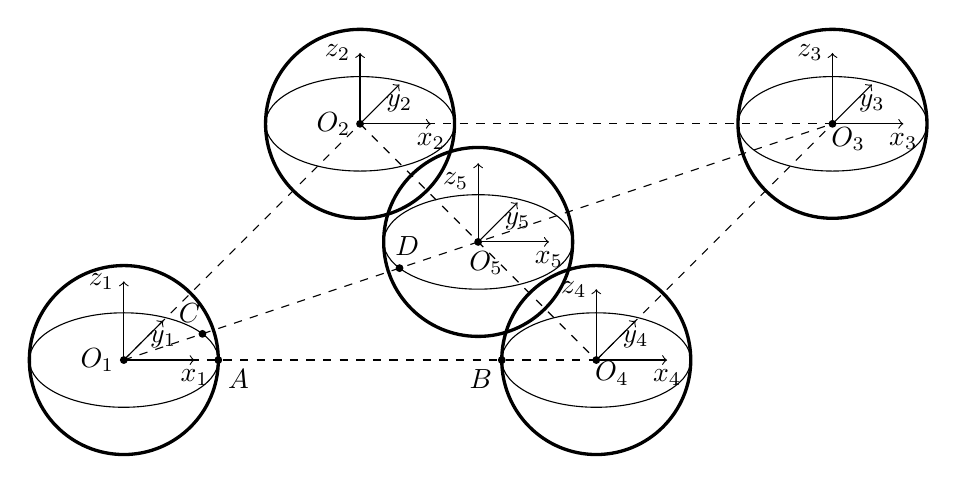
\begin{tikzpicture}%[scale=1.5]
  \draw[->] (0,0) -- (0.9,0) node[anchor=north] {$x_1$};
  \draw[->] (0,0) -- (0,1) node[anchor=east] {$z_1$};
  \draw[->] (0,0) -- (0.5,0.5) node[anchor=north] {$y_1$};
  \draw[->] (6.0,0) -- (6.9,0) node[anchor=north] {$x_4$};
  \draw[->] (6.0,0) -- (6.0,0.9) node[anchor=east] {$z_4$};
  \draw[->] (6.0,0) -- (6.5,0.5) node[anchor=north] {$y_4$};
  \draw[->] (3,3) -- (3.9,3) node[anchor=north] {$x_2$};
  \draw[->] (3,3) -- (3,3.9) node[anchor=east] {$z_2$};
  \draw[->] (3,3) -- (3.5,3.5) node[anchor=north] {$y_2$};
  \draw[->] (9,3) -- (9.9,3) node[anchor=north] {$x_3$};
  \draw[->] (9,3) -- (9,3.9) node[anchor=east] {$z_3$};
  \draw[->] (9,3) -- (9.5,3.5) node[anchor=north] {$y_3$};
  \draw[->] (4.5,1.5) -- (5.4,1.5) node[anchor=north] {$x_5$};
  \draw[->] (4.5,1.5) -- (4.5,2.5) node[anchor=north east] {$z_5$};
  \draw[->] (4.5,1.5) -- (5.0,2.0) node[anchor=north] {$y_5$};

  \node[left] at (0,0) {$O_1$};
  \node[left] at (3,3) {$O_2$};
  \node[below] at (6.2,0.1) {$O_4$};
  \node[below] at (9.2,3.08) {$O_3$};
  \node[below] at (4.6,1.5) {$O_5$};
  \node[below right] at (1.2,0) {$A$};
  \node[below left] at (4.8,0) {$B$};
  \node[above left] at (1.1,0.35) {$C$};
  \node[above] at (3.6,1.2) {$D$};

  \draw[very thick] (0,0) circle (1.2);
  \draw (0,0) ellipse (1.2 and .6);

  \draw[very thick] (6.0,0) circle (1.2);
  \draw (6.0,0) ellipse (1.2 and .6);

  \draw[very thick] (3,3) circle (1.2);
  \draw (3,3) ellipse (1.2 and .6);

  \draw[very thick] (9,3) circle (1.2);
  \draw (9,3) ellipse (1.2 and .6);

  \draw[very thick] (4.5,1.5) circle (1.2);
  \draw (4.5,1.5) ellipse (1.2 and .6);

%  \draw (0,0) -- (2.5,2);
%  \draw[dashed] (2.5,2) -- (2.5,-2.5);
%  \draw[dashed] (0,0) -- (2.5,-2.5);

  \node[circle, fill=black, inner sep=1pt] at (0,0) {};
  \node[circle, fill=black, inner sep=1pt] at (3,3) {};
  \node[circle, fill=black, inner sep=1pt] at (6,0) {};
  \node[circle, fill=black, inner sep=1pt] at (9,3) {};
  \node[circle, fill=black, inner sep=1pt] at (4.5,1.5) {};
  \node[circle, fill=black, inner sep=1pt] at (1.2,0) {};
  \node[circle, fill=black, inner sep=1pt] at (4.8,0) {};
  \node[circle, fill=black, inner sep=1pt] at (0.99846,0.33282) {};
  \node[circle, fill=black, inner sep=1pt] at (3.50154,1.16718) {};
  
  \draw[dashed] (0,0) -- (6,0);
  \draw[dashed] (0,0) -- (3,3);
  \draw[dashed] (3,3) -- (9,3);
  \draw[dashed] (6,0) -- (9,3);
  \draw[dashed] (3,3) -- (6,0);
  \draw[dashed] (0,0) -- (9,3);
\end{tikzpicture}
\end{document}

%%% Local Variables: 
%%% mode: latex
%%% TeX-master: t
%%% End: 
